\documentclass{beamer}c
\usepackage[utf8]{inputenc}
\usepackage[spanish,es-tabla]{babel}
\usepackage{graphicx}
\graphicspath{ {imagenes/} }

\usetheme{PaloAlto}

\title{An Efficient Parallel Algorithm for Secured Data Communications Using RSA Public Key Cryptography Method}

\author{Christofer Chávez Carazas}


\institute[Universidad Nacional de San Agustín] 


\date{\today}

\subject{Proyectos I}
\AtBeginSubsection[]
{
  \begin{frame}<beamer>{Outline}
    \tableofcontents[currentsection,currentsubsection]
  \end{frame}
}

\begin{document}

\begin{frame}
  \titlepage
\end{frame}

\begin{frame}{Motivación}
  \begin{itemize}
   \item Utilizar \textit{GNU MP} para realizar las operaciones con enteros grandes que requiere el \textit{RSA}.
   \item Paralelizar la exponenciación modular con \textit{OpenMP} para reducir el tiempo de encriptado y desencriptado.
   del \textit{RSA}
  \end{itemize}
\end{frame}

\begin{frame}{RSA}
 \begin{itemize}
  \item Sistema criptográfico asimétrico.
  \item Producto de dos números primos grandes.
  \item Usa al exponenciación modular.
 \end{itemize}
\end{frame}

\begin{frame}{Generación de llaves}
  \begin{enumerate}
   \item Se escogen aleatoriamente dos números primos grandes \textit{q} y \textit{p}.
   \item Se obtiene el módulo $n = q * p$.
   \item Se calcula  $\varphi(n) = (p-1)(q-1)$
   \item Se selecciona un \textit{e} que cumpla: $1 < e < \varphi(n)$ y que sea coprimo con $\varphi(n)$.
   \item Se selecciona un \textit{d} que cumpla: $1 < d < \varphi(n)$ tal que $e*d = 1\:mod\:\varphi(n)$.
  \end{enumerate}
\end{frame}

\begin{frame}{Cifrado y Descifrado}
  \begin{block}{Cifrado}
    $$c \equiv m^{e} (mod\:n)$$ 
    Donde \textit{c} es el mensaje cifrado, \textit{m} es el mensaje original, \textit{e} es la llave pública y
    \textit{n} es el módulo hallado anteriormente.
  \end{block}
  \begin{block}{Descifrado}
   $$m \equiv c^{d} (mod\:n)$$
   Donde \textit{m} es el mensaje original, \textit{c} es el mensaje cifrado, \textit{d} es la llave privada y
   \textit{n} es el módulo hallado anteriormente.
  \end{block}
\end{frame}

\begin{frame}{Repeated square-and-multiply Algorithm}
  El algoritmo se basa en la siguiente observación:
  $$g^{e} mod\:m = (g^{e/2} * g^{e/2}) mod\:m$$
  y se puede definir recursivamente de la siguiente manera:
  \begin{figure}
   \centering
   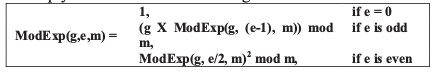
\includegraphics[scale = 0.5]{1.png}
   \caption{\textit{Repeated square-and-multiply} \cite{Paper}}
   \label{fig:1}
  \end{figure}
\end{frame}

\begin{frame}{Exponenciación Modular binaria Paralela}
\begin{itemize}
 \item Se convierte el exponente a su forma binaria y se lo divide en k partes dependiendo del número de procesadores.
 \item La exponenciación tendría la siguiente forma:
 $$g^{e} = g^{2^{r_{k}}e_{k}} \cdots g^{2^{r_{2}}e_{2}}*g^{2^{r_{1}}e_{1}}$$
 siendo las \textit{r} calculadas de la siguiente forma:
 $$r_{1} = 0, r_{2} = \frac{n}{k}, r_{3} = \frac{2n}{k},\cdots,r_{k} = \frac{(k-1)n}{k}$$
 \item Cada parte se calcula con el \textit{Repeated square-and-multiply Algorithm}
\end{itemize}
\end{frame}

\begin{frame}{Experimentos - Test Case Sets}
  \begin{block}{Test Case Set 1}
   \begin{itemize}
    \item Diferentes tamaños de llaves: 128, 256, 512, 768, 1024 y 2048 bits.
    \item Mismo tamaño de mensaje: 5000 caracteres.
   \end{itemize}
  \end{block}
  \begin{block}{Test Case Set 2}
   \begin{itemize}
    \item Mismo tamaño de llaves: 1024 bits.
    \item Diferentes tamaños de mensaje: 1000, 2000, 3000, 4000, 5000 y 6000 caracteres.
   \end{itemize}
  \end{block}
\end{frame}

\begin{frame}{Experimentos}
   \begin{itemize}
    \item Se tomó el tiempo de cifrado, descifrado y las suma de los dos anteriores más el tiempo
    que demora la generación de llaves
    \item Para cada caso se corrió el programa 25 veces y se sacó el tiempo promedio.
    \item Se calculó el \textit{speedup} para los casos con 8 threads.
   \end{itemize}
\end{frame}

\begin{frame}{Experimentos - Resultados - Set 1}
  \begin{table}
  \begin{figure}
   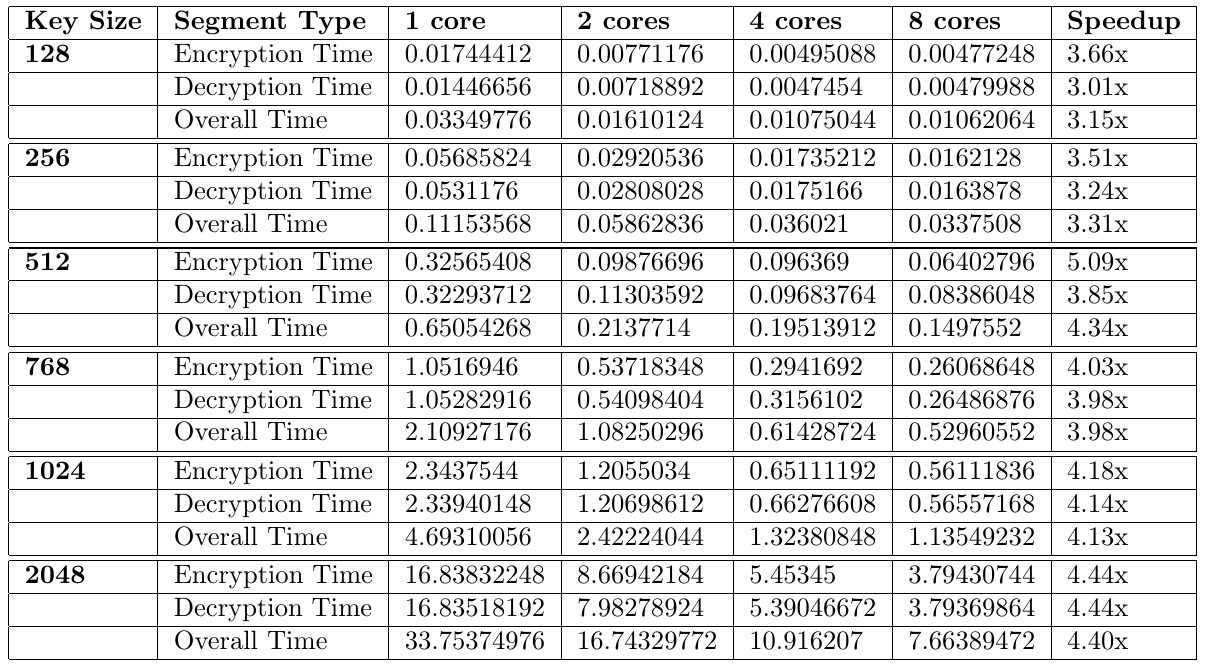
\includegraphics[scale = 0.25]{2.png}
  \end{figure}
  \caption{Resultados con el \textit{Set 1}}
  \end{table}
\end{frame}

\begin{frame}{Experimentos - Resultados - Set 2}
  \begin{table}
   \begin{figure}
    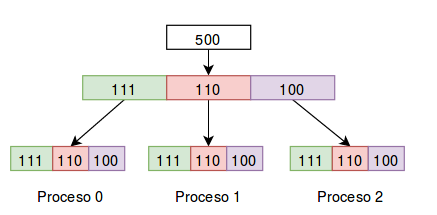
\includegraphics[scale = 0.24]{3.png}
   \end{figure}
  \caption{Resultados con el \textit{Set 2}}
  \end{table}

 
\end{frame}


\begin{frame}
\begin{thebibliography}{}
\setbeamertemplate{bibliography item}[article]
\bibitem[S. Saxena et al. 2014]{Paper} Sapna Saxena, Bhanu Kapoor \textbf{An Efficient Parallel Algorithm for Secured Data Communications Using RSA Public Key Cryptography Method}, 2014.
\end{thebibliography}
\end{frame}

\end{document}


